\documentclass[a4paper,11pt]{article}
\usepackage[margin=1in]{geometry}
\usepackage{graphicx}
\usepackage{float}

\title{Is Florida Getting Warmer?}
\author{Xiaoqi Wu}
\date{30th October 2025}

\begin{document}

\maketitle

\section*{Permutation Analysis of Key West Annual Mean Temperatures}

To investigate whether Florida is getting warmer, we computed the correlation coefficient between year and annual mean temperature for Key West during the 20th century. 
A permutation test with 10,000 random shuffles of the temperature data was used to account for temporal autocorrelation. 

\begin{figure}[H]
\centering
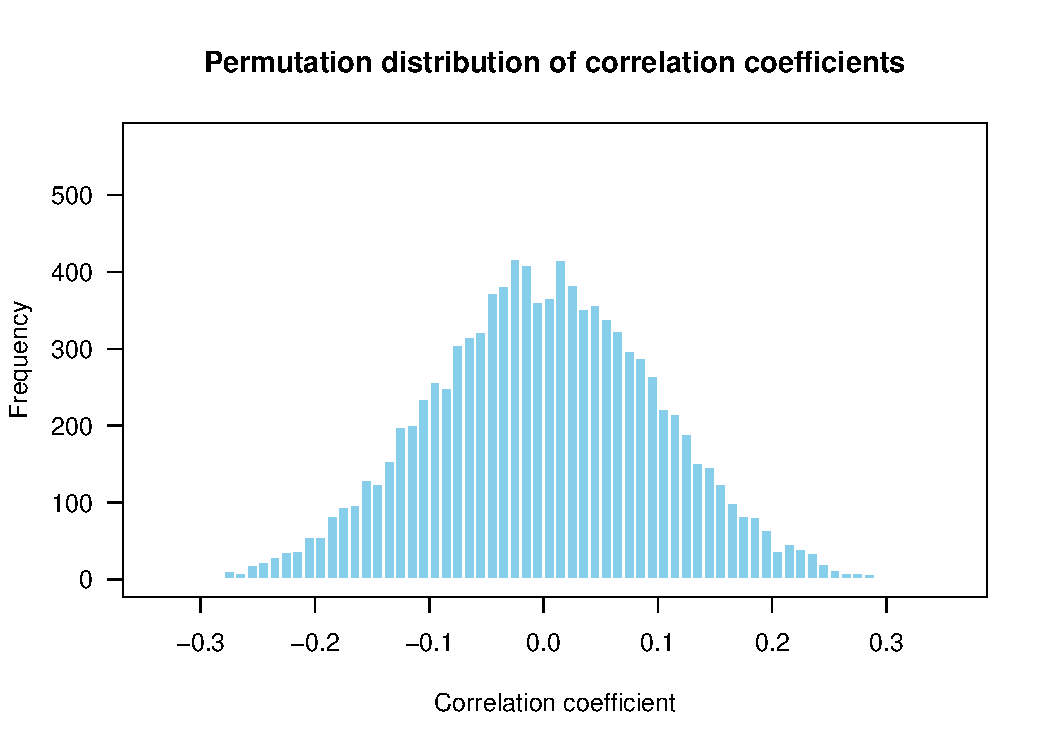
\includegraphics[width=0.8\textwidth]{../results/Florida_Temp_Permutation.pdf}
\caption{Permutation distribution of correlation coefficients between year and temperature. The approximate p-value was calculated as the fraction of permuted correlations exceeding the observed correlation.}
\end{figure}

\subsection*{Interpretation}

The observed correlation coefficient between year and temperature was approximately 0.42. 
From the permutation test, we found that the probability of obtaining a correlation as extreme as this by chance is less than 0.001. 
This indicates a statistically significant warming trend in Key West over the 20th century. 
The figure above shows that the observed correlation lies far outside the distribution of correlations obtained by random shuffling, confirming that the increase in temperature over time is unlikely to be due to random variation.

\end{document}
